\documentclass[12pt,a4paper,ngerman,captions=tableheading]{scrartcl}

% -----------------------------------------------
% --------PAKETE-LADEN---------------------------
% -----------------------------------------------
\usepackage{rotating}
\usepackage{acronym}
\usepackage{graphicx}
\usepackage{longtable}
\usepackage{booktabs}


% -----------------------------------------------
% --------Seitengeometrie------------------------
% -----------------------------------------------

\usepackage{geometry}
\geometry{a4paper, top=27mm, left=30mm, right=20mm, bottom=35mm, headsep=10mm, footskip=12mm}

% -----------------------------------------------
% --------Schrift-+-Wörterbuch-------------------
% -----------------------------------------------

\usepackage[T1]{fontenc}
\usepackage[utf8]{inputenc}
\usepackage{babel}
\usepackage{lmodern}

\usepackage{microtype}
    % \setlength{\emergencystretch}{1em}

\usepackage[scaled]{helvet}
    % Serifenfreie Schrift: 
    % \renewcommand{\familydefault}{\sfdefault}

    % Zeilenabsatz - Einrücken verhindern:
\setlength{\parindent}{0em} 

    % Zeilenabstand auf 1,5: 
\usepackage[onehalfspacing]{setspace}


%------------------------------------------------------
%-----KOPF-und-FUSSZEILEN------------------------------
%------------------------------------------------------

\usepackage{scrlayer-scrpage}
%\usepackage[headtopline,headsepline]{scrlayer-scrpage}
%\setheadtopline{0,4pt}
%\setheadsepline{}

\clearpairofpagestyles
\ihead{ Spezielle Messtechnik (MST2) }
\chead{SAM}
\ohead{\today}
\ifoot*{}
\ofoot{\pagemark}
\pagestyle{scrheadings}
\setkomafont{pageheadfoot}{\small}
\setkomafont{pagehead}{}
\usepackage{breakurl}


%------------------------------------------------------
%--------Physik und Mathe------------------------------
%------------------------------------------------------

\usepackage{upgreek}

\usepackage{chemformula}


\usepackage{chemmacros}

    

\usepackage{mathtools} % lädt auch amsmath

\usepackage{amssymb}
    % & vor entsprechendem Zeichen richtet nachfolgende Formeln daran aus
    % Leerzeilen beenden den Modus! 

\usepackage{siunitx}
\sisetup{inter-unit-product = \cdot}
\sisetup{detect-family}

    % detect-weight, % Schrifttyp übernehmen (bold, kursiv etc) 
    % detect-family, %Schriftart des Umgebungstextes übernehmen (mit/ohne Serifen) 
\DeclareUnicodeCharacter{2212}{-}

% -----------------------------------------
% ---------Links--------------------------------
% -----------------------------------------

\usepackage{url}
\urlstyle{same}



% -----------------------------------------
% -------Listen --------------------------------
% -----------------------------------------

\usepackage{mdwlist}
\usepackage{paralist}

% -------------------------------------------------------------
% Tabellen und Grafiken--------------------------------
% -------------------------------------------------------------
\usepackage{makecell}
\usepackage{graphicx}
\usepackage[lofdepth,lotdepth]{subfig}
%\usepackage{subfigure}
\usepackage{pdfpages}
\usepackage{float}
\usepackage{pdflscape}
\usepackage{tabularx}
\newcolumntype{L}[1]{>{\raggedright\arraybackslash}m{#1}} % linksbündig mit Breitenangabe
\newcolumntype{C}[1]{>{\centering\arraybackslash}m{#1}} % zentriert mit Breitenangabe
\newcolumntype{R}[1]{>{\raggedleft\arraybackslash}m{#1}} % rechtsbündig mit Breitenangabe

\usepackage{multirow}
\usepackage{array}
\usepackage{colortbl}
\definecolor{MKHgreen}{RGB}{65, 160, 55}
\usepackage{tikz}
\usetikzlibrary{external}
%\tikzexternalize
\usepackage{adjustbox}
\usepackage{pgfplots}
\usepgfplotslibrary{colorbrewer}
\pgfplotsset{compat = newest} 
% Tikz is loaded automatically by pgfplots
\usetikzlibrary{pgfplots.statistics, pgfplots.colorbrewer} 
% provides \pgfplotstabletranspose
\usepackage{pgfplotstable}
\usepackage{filecontents}

\usepackage{framed}
\usepackage{xcolor}
\colorlet{shadecolor}{gray!25}
    %\begin{shaded}
    %\end{shaded}



    %Bildunterschriften // justification=raggedright längere Bildunterschriften/Tabellenüberschriften werden linksbündig ausgerichtet, singlelinecheck=false auch kurze Bildunterschriften/Tabellenüberschriften werden linksbündig ausgerichtet
    
\usepackage{caption}
\usepackage{subcaption}
%\usepackage[labelfont=bf,font={small,sf},justification=raggedright,singlelinecheck=false]{caption} 
\addto\captionsngerman{\renewcommand{\figurename}{Abb.}}
\addto\captionsngerman{\renewcommand{\tablename}{Tab.}}


%------------------------------------------------------
%-----HYPERREF-----------------------------------------
%------------------------------------------------------

\usepackage[
  colorlinks, 
  backref=true, 
  pdfpagelabels, 
  pdfstartview=FitH, 
  bookmarksopen=true, 
  bookmarksnumbered=true, 
  pdftitle={Berichte}, 
  pdfauthor={Ahmed EN-NOUR}, 
  pdfsubject={MST}, 
  pdfcreator={}, 
  pdfproducer={}, 
  pdfkeywords={MST, Messung, Labor}, 
  pdfnewwindow=true, 
  linkcolor=black, 
  plainpages=false, 
  hypertexnames=false, 
  citecolor=black, 
  filecolor=black, 
  urlcolor=black
]{hyperref}


    % Links auf Gleitumgebungen springen nicht zur Beschriftung, sondern zum Anfang der Gleitumgebung:

\usepackage[figure,table]{hypcap}

    % \usepackage[table]{hypcap}
    % oder  
    % \usepackage[tabularx]{hypcap}
    

\usepackage[labelfont=bf,justification=RaggedRight,textfont=it]{caption}
\DeclareCaptionLabelSeparator{period-newline}{. \newline}

%------------------------------------------------------
%-----LITERATURQUELLEN---------------------------------
%------------------------------------------------------

\usepackage[babel, german=quotes]{csquotes}
\usepackage[
backend=biber,
style=numeric,
sorting=none
]{biblatex}
\addbibresource{quellen.bib}
\renewcommand*{\bibfont}{\normalfont}


\usepackage{wrapfig}
\graphicspath{{./images/}}

    % Passt die Schriftgröße  im Quellenverzeichnis an die Normale Schriftgröße an:



\sisetup{output-decimal-marker = {,}}
\pgfkeys{/pgf/number format/use comma}


%------------------------------------------------------
%-----NUMMERIERUNG-------------------------------------
%------------------------------------------------------

\setcounter{secnumdepth}{3}
\usepackage{multirow}
%------------------------------------------------------
%-----WORTTRENNUNG-------------------------------------
%------------------------------------------------------

\usepackage{pgfplots}
\pgfplotsset{width=10cm,compat=1.9,every mark/.append style={solid},}
%\pgfplotsset{every mark/.append style={solid},}


% We will externalize the figures
\usepgfplotslibrary{external}

\hyphenation{Tren-nungs-kor-rek-tur}


%\usepackage[Labor=true,backref=true]{hyperref}
%------------------------------------------------------
%------------------DOKUMENT----------------------------
%------------------------------------------------------

\begin{document}

%------------------------------------------------------
%------------------Titelseite--------------------------
%------------------------------------------------------

\begin{titlepage}
\centering
\begin{onehalfspace}
    \huge \textbf{}  
    \linebreak \large \textbf{}
\end{onehalfspace}

%------------------------------------------------------
%------------------------Logo--------------------------
%------------------------------------------------------


\includegraphics[height=70pt]{Bilder/fhkiel_logo.jpg}

\vspace{0.6cm}

\begin{onehalfspace}
    \huge \textbf{Spezielle Messtechnik (MST2) – Labor}  \linebreak \large \textbf{}
\end{onehalfspace}

\vspace{0.3cm}

\begin{onehalfspace}
    \Large \textbf{Laborversuch V3: SAM}
\end{onehalfspace}

\vspace{1cm}
{\large Teilnehmer:} 
%{\large vorgelegt von:}
    \vspace{0.5cm}

    \begin{tabular}{l l}
        \large\textbf{Alaa Albasha}, & \textbf{Matr. Nr.: 943167} \\
        \large\textbf{Jan-Manuel Megerle}, & \textbf{Matr. Nr.: 942883} \\
        \large\textbf{Nathan Kirori}, & \textbf{Matr. Nr.: 941689} \\
        \large\textbf{Ahmed EN-NOUR}, & \textbf{Matr. Nr.: 937048} \\
    \end{tabular}


    

    \vspace{0.5cm}
    
\large \textbf{MST2\_M2 - Team 1}

\vspace{1cm}
{\large Professor:}

    \vspace{0.2cm}
    
\large \textbf{Prof. Dr.-Ing. Aylin Bicakci }

    \vspace{0.3cm}

\large \textbf{Fachhochschule Kiel \linebreak Sommersemester 2025\\}
{\large Informatik und Elektrotechnik}

\vfill
%\begin{center}
 %       28.10.2023
%\end{center}
\end{titlepage}


\newpage

%------------------------------------------------------
%------------------INHALTSVERZEICHNIS------------------
%------------------------------------------------------

\tableofcontents  
%\textbf{Anhang}
\newpage

%------------------------------------------------------
%------------------INHALT----------------------------
%------------------------------------------------------

\section{Einleitung}
In dem letzten Versuch wurde die Anwendung des Rasterelektronenmikroskops (REM) dargestellt und erklärt. Allerdings tritt häufig das Problem auf, dass einige Proben in den inneren Schichten Schäden aufweisen, die mit dem REM nicht erkennbar sind, da es lediglich die Oberfläche analysieren kann.\\ An dieser Stelle kommt die SAM-Technologie (Scanning Acoustic Microscopy) zum Einsatz, da sie mithilfe von Ultraschallwellen die innere Struktur der Schichten sichtbar machen kann. In diesem Versuch wird dies nun durch praktische Anwendung bewiesen..


%------------------------------------------------------
%######################################################
%------------------------------------------------------

\section{Theoretische Grundlagen}
Die Scanning Acoustic Microscope (SAM), auch bekannt als akustisches Mikroskop, wurde 1974 an der Stanford University entwickelt und stellte das erste Instrument dar, das in der Lage war, ein akustisches Bild zu erzeugen.\\

Das Grundprinzip der SAM basiert auf einem Wandler (Transducer), der Ultraschallwellen erzeugt. Diese werden mithilfe einer akustischen Linse fokussiert und auf die zu untersuchende Probe gerichtet. Beim Auftreffen auf das Material werden die Wellen absorbiert, reflektiert oder gestreut, abhängig von den Eigenschaften der inneren Strukturen. Die reflektierten Wellen werden von Detektoren – meist oberhalb oder unterhalb der Probe – erfasst und in elektrische Signale umgewandelt.

Diese elektrischen Signale liefern Informationen über materialinterne Eigenschaften wie Schichtdicke, Dichte und Grenzflächenbeschaffenheit. Die verwendeten Frequenzen der Ultraschallwellen sind dabei entscheidend, da sie die Auflösung und Eindringtiefe bestimmen. Je nach Frequenz können innere Strukturen wie Risse, Delaminationen, Lufteinschlüsse oder Hohlräume detektiert werden.

Eine Vielzahl von Materialien, die in der industriellen Fertigung verwendet werden – etwa Silizium, Epoxidharz, Bonding-Materialien und Metallrahmen – übertragen Ultraschallwellen ausreichend gut, um eine bildgebende Analyse zu ermöglichen.\\

Das am häufigsten genutzte Verfahren der SAM ist der Reflexionsmodus (Pulse-Echo-Verfahren). Dabei wird eine Ultraschallwelle in die Probe eingekoppelt. Ein Teil der Welle wird an inneren Grenzflächen reflektiert und gelangt zurück zum Wandler, wo sie erneut in ein elektrisches Signal umgewandelt wird. Die Intensität und Polarität dieser Signale liefern Rückschlüsse auf die inneren Strukturen des untersuchten Materials.
\\



 \newpage
\vspace{0.2cm}
\begin{figure}
    \centering
    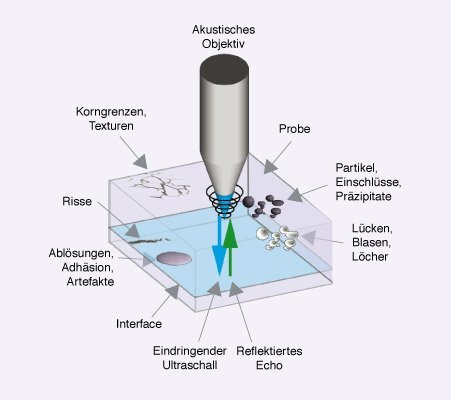
\includegraphics[scale=0.8]{Bilder/samtheorie}
    \caption{Schematische Darstellung des Funktionsprinzips der Scanning Acoustic Microscopy (SAM) im Reflexionsmodus. Die eingestrahlten Ultraschallwellen werden an inneren Strukturen wie Rissen, Grenzflächen, Einschlüsse oder Delaminationen reflektiert und ermöglichen so eine zerstörungsfreie Analyse der Probe.}
    \par Quelle: \href{https://www.pvatepla-lwt.com/technologien/funktionsweise-der-ultraschallmikroskopie/}{PVA Tepla: SAM funktionsweise}
    \vspace{0.2cm}
    \label{Abb.1: Schematische Darstellung des Funktionsprinzips der Scanning Acoustic Microscopy (SAM) im Reflexionsmodus. Die eingestrahlten Ultraschallwellen werden an inneren Strukturen wie Rissen, Grenzflächen, Einschlüsse oder Delaminationen reflektiert und ermöglichen so eine zerstörungsfreie Analyse der Probe. }
\end{figure} 
\vspace{0.2cm}
Zur optimalen Übertragung der akustischen Wellen befindet sich die Probe während der Messung in einem Wasserbad. Wasser dient dabei als Kopplungsmedium, da es eine homogene akustische Impedanz aufweist und eine gleichmäßige Grenzfläche zwischen Sonde und Probe bildet.


%------------------------------------------------------
%######################################################
%------------------------------------------------------

%\newpage
\section{Aufgabenstellung}
In diesem Versuch wird die akustische Mikroskopie (SAM) eingesetzt, um zu demonstrieren, wie eine zerstörungsfreie bildgebende Untersuchung innerer Strukturen in Materialien durchgeführt werden kann. Dabei sollen insbesondere potenzielle Defekte wie Risse, Delaminationen, Lufteinschlüsse oder andere strukturelle Schäden identifiziert und analysiert werden.
Die Untersuchung erfolgt an drei verschiedenen Proben, bei denen gezielt geeignete Untersuchungsebenen gewählt werden müssen, um relevante Fehlstellen sichtbar zu machen. Ziel ist es, auffällige Bereiche zu dokumentieren, die jeweiligen Fehlerarten zu identifizieren und deren Ursache sowie Auswirkungen auf die Materialstruktur zu erläutern.

%------------------------------------------------------
%######################################################
%------------------------------------------------------

%

%------------------------------------------------------
%######################################################
%------------------------------------------------------

\section{Proben und Methoden}
Zunächst wird die akustische Mikroskopie verwendet, um darstellen zu können, wie eine Zerstörung freie Untersuchung erfolgen kann, darüber hinaus werden nach Risse und irgendwelche Schaden untersucht und mögliche Darstellung bemerken zu können wie Luftblasen. Diese Untersuchung wird mit drei Proben durchgeführt.
Aufgabe bei den Proben ist auch die Ebenen zu wählen, die für eine solchen Untersuchung sinnvoll sind.  Potentielle
Defekte oder Fehler müssen dokumentiert und erläutert werden.


In diesem Experiment werden drei unterschiedliche Proben mit dem KSI V8 SAM untersucht, um innere Strukturen und Defekte zerstörungsfrei zu erkennen. Die Messung erfolgt im Reflexionsmodus, wobei Ultraschallwellen über ein Wasserbad eingekoppelt und reflektierte Signale ausgewertet werden.

Die erste Probe ist eine keramische DCB-Leiterplatte mit gesinterten Halbleitern, teils mit Bonddrähten kontaktiert (siehe Abbildung 3). Sie dient zur Einführung in die SAM-Bedienung und zur Darstellung verschiedener Materialübergänge in mehreren Ebenen.

Die zweite Probe besteht aus einem Kupfer-Leadframe, der auf ein keramisches Substrat geschweißt wurde (siehe Abbildung 4). Hier liegt der Fokus auf der Analyse der Schweißverbindungen und der Untersuchung möglicher Defekte durch Wahl geeigneter Scanebenen.

Die dritte Probe ist ein DoL-Leistungselektronikmodul ohne Bonddrähte (siehe Abbildung 5). Statt keramischer Isolation kommt eine organische Trägerfolie zum Einsatz. Die Ebenenwahl und Bewertung erfolgen selbstständig.

Alle Proben werden im Wasserbecken positioniert, wobei auf die Entfernung von Luftblasen geachtet wird. Die Steuerung erfolgt über den integrierten PC, und nach jeder Messung wird das Gerät in die Home-Position zurückgefahren.



Die Untersuchung erfolgt mit dem Scanning Acoustic Microscope KSI V8 \cite{2}, einem Hochleistungsgerät zur zerstörungsfreien Prüfung und Fehleranalyse in Bereichen wie der Mikroelektronik, Materialwissenschaft und Halbleiterfertigung. Das Gerät arbeitet im Frequenzbereich von 5MHz bis 400MHz, wodurch sich die Eindringtiefe und Auflösung flexibel an das zu untersuchende Material anpassen lassen. Mit einer Scangeschwindigkeit von bis zu 2m/s und einer Positionsgenauigkeit von 1m ermöglicht der KSI V8 eine präzise und gleichzeitig zeiteffiziente Analyse.

Das System bietet mehrere Scanmodi, die eine detaillierte Untersuchung unterschiedlicher Strukturen ermöglichen. Im sogenannten C-Scan-Modus wird eine zweidimensionale Darstellung einer definierten Fokusebene erzeugt, die sich besonders zur Erkennung von Hohlräumen und Rissen innerhalb einzelner Materialschichten eignet. Ergänzend dazu erlaubt der B-Scan die Darstellung eines Tiefenprofils, während der 3D-Scan durch die Kombination mehrerer Ebenen eine volumetrische Abbildung des Probenaufbaus liefert.


\begin{figure}[htbp]
    \centering
    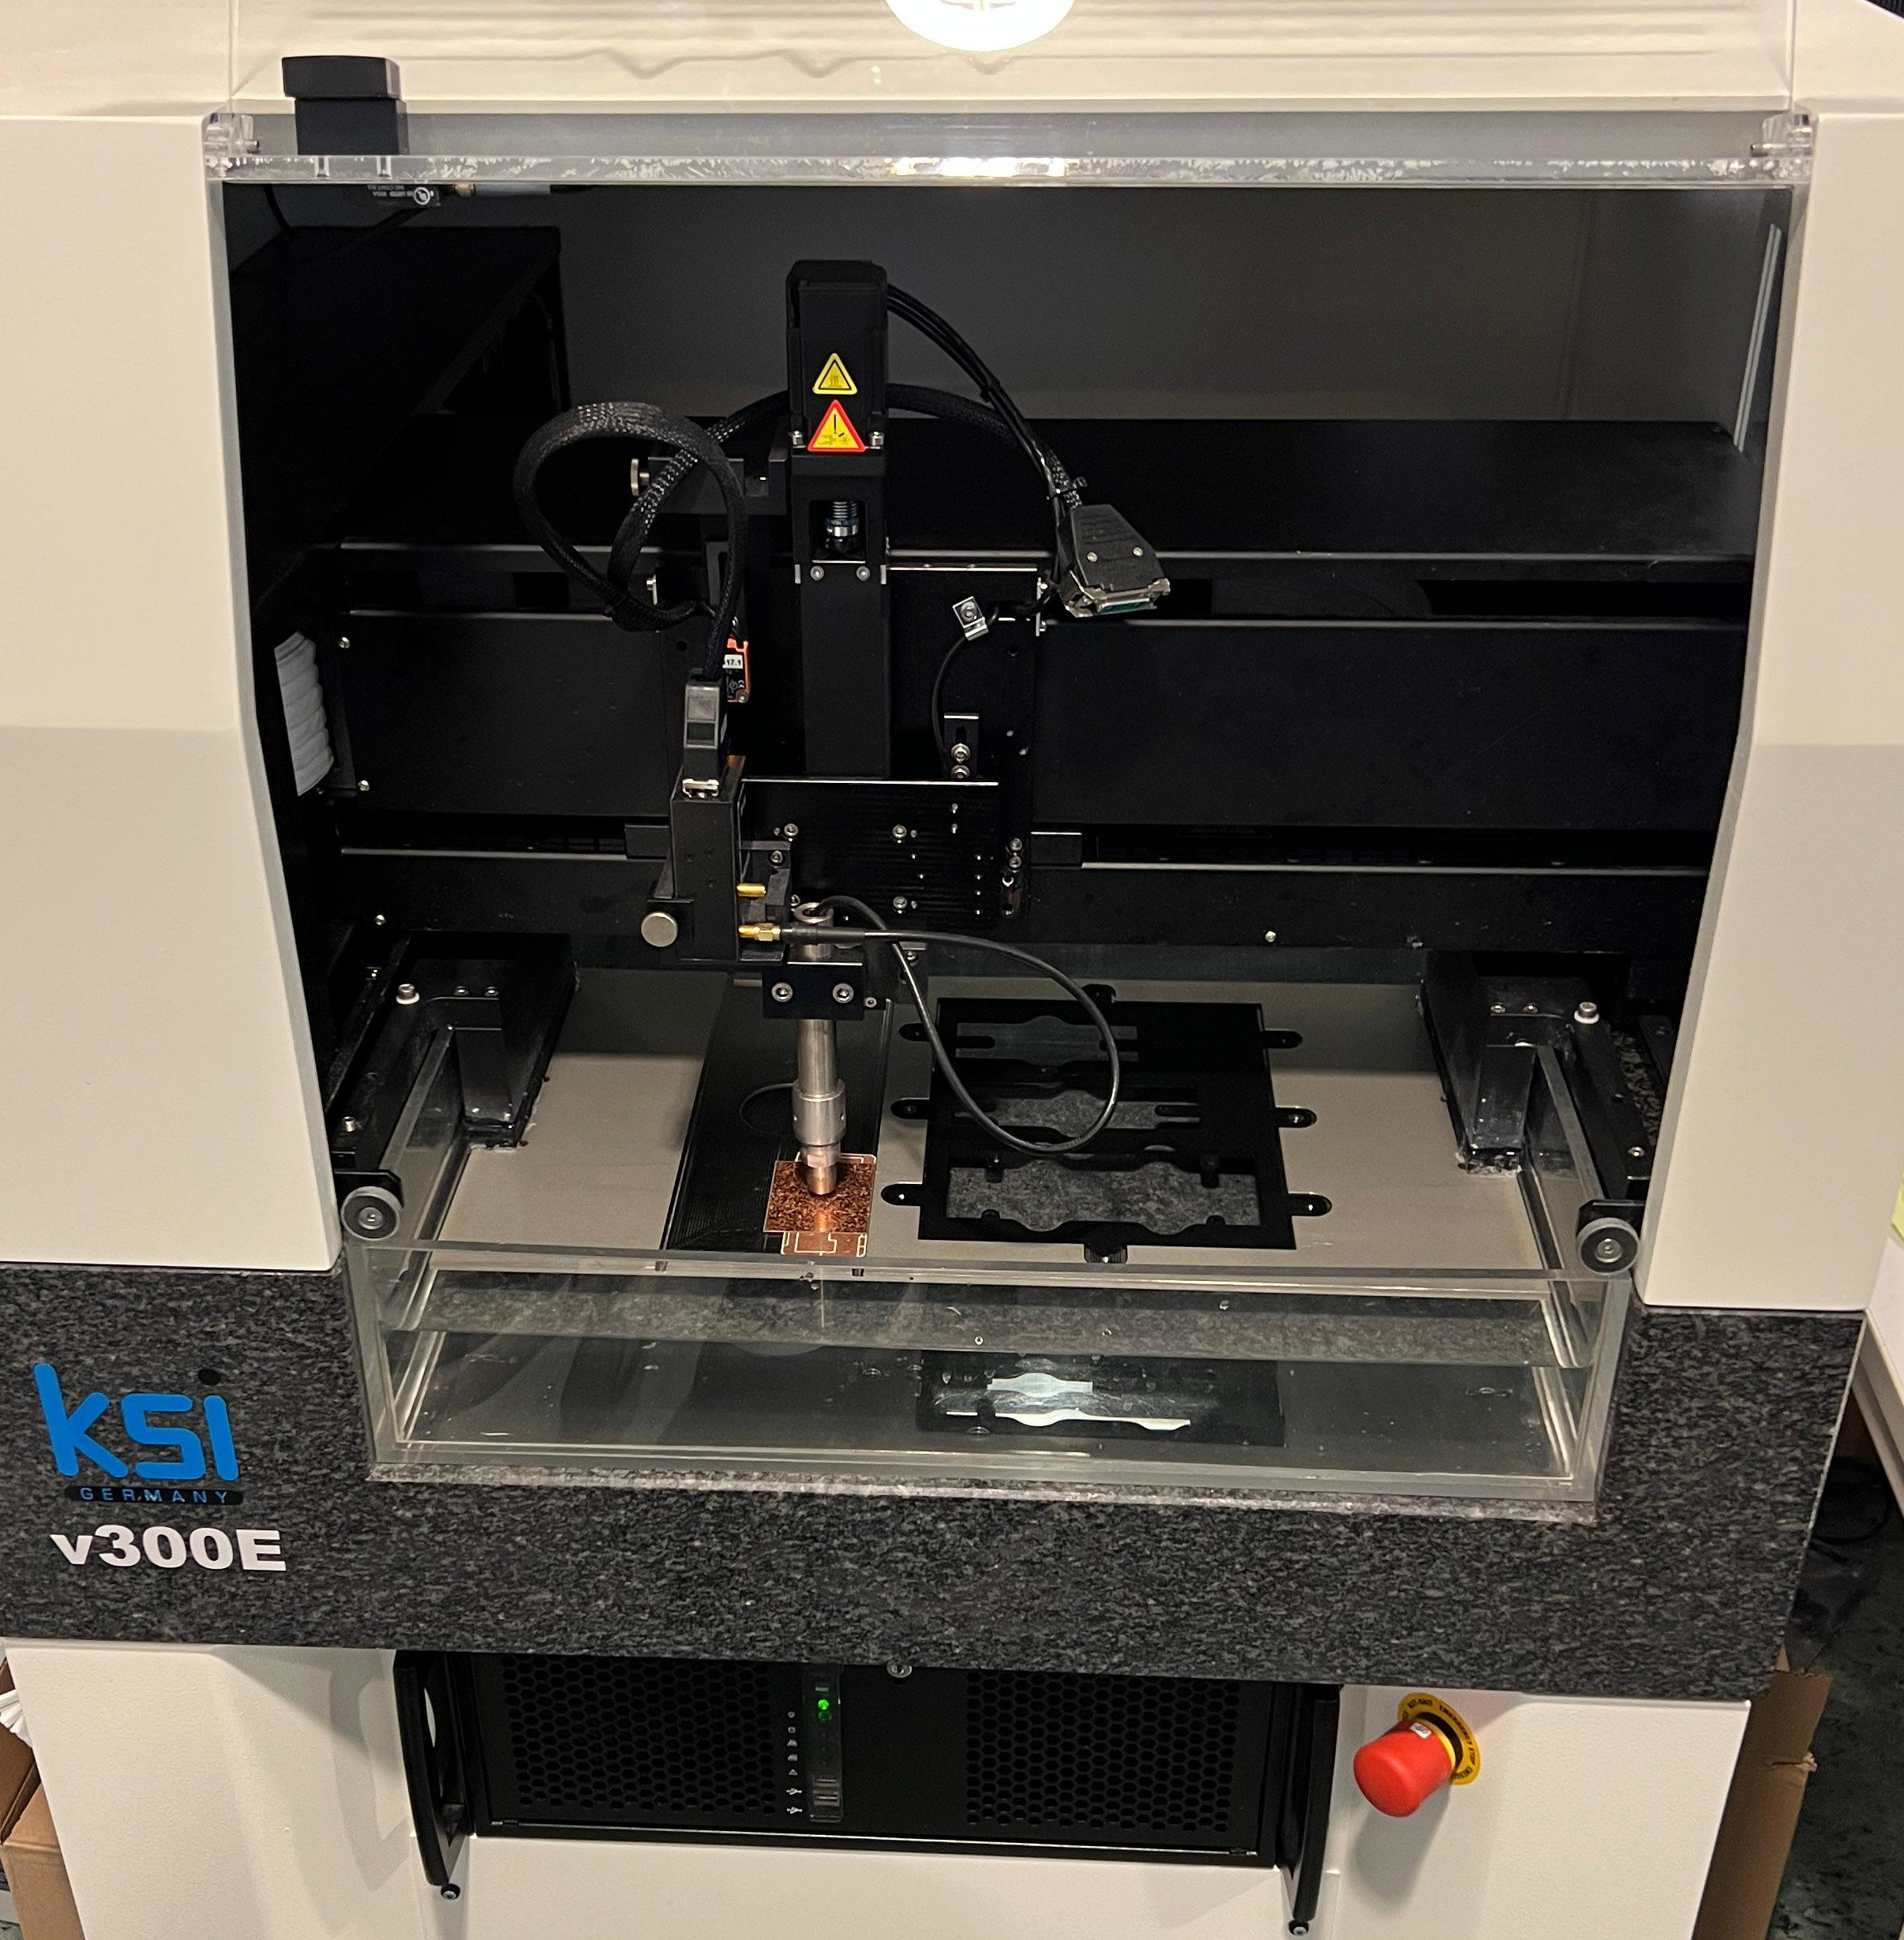
\includegraphics[scale=0.11]{Bilder/ksiv8}
    \caption{KSI v300E Ultraschallmikroskop am Messplatz. Die Probe wird in einem Wasserbad positioniert und mittels eines piezoelektrischen Wandlers im Reflexionsmodus untersucht.}
    \vspace{0.2cm}
    \label{Abb.2: KSI v300E Ultraschallmikroskop am Messplatz. Die Probe wird in einem Wasserbad positioniert und mittels eines piezoelektrischen Wandlers im Reflexionsmodus untersucht. }
\end{figure} 
\vspace{0.2cm}
\begin{figure}[htbp]
    \centering
    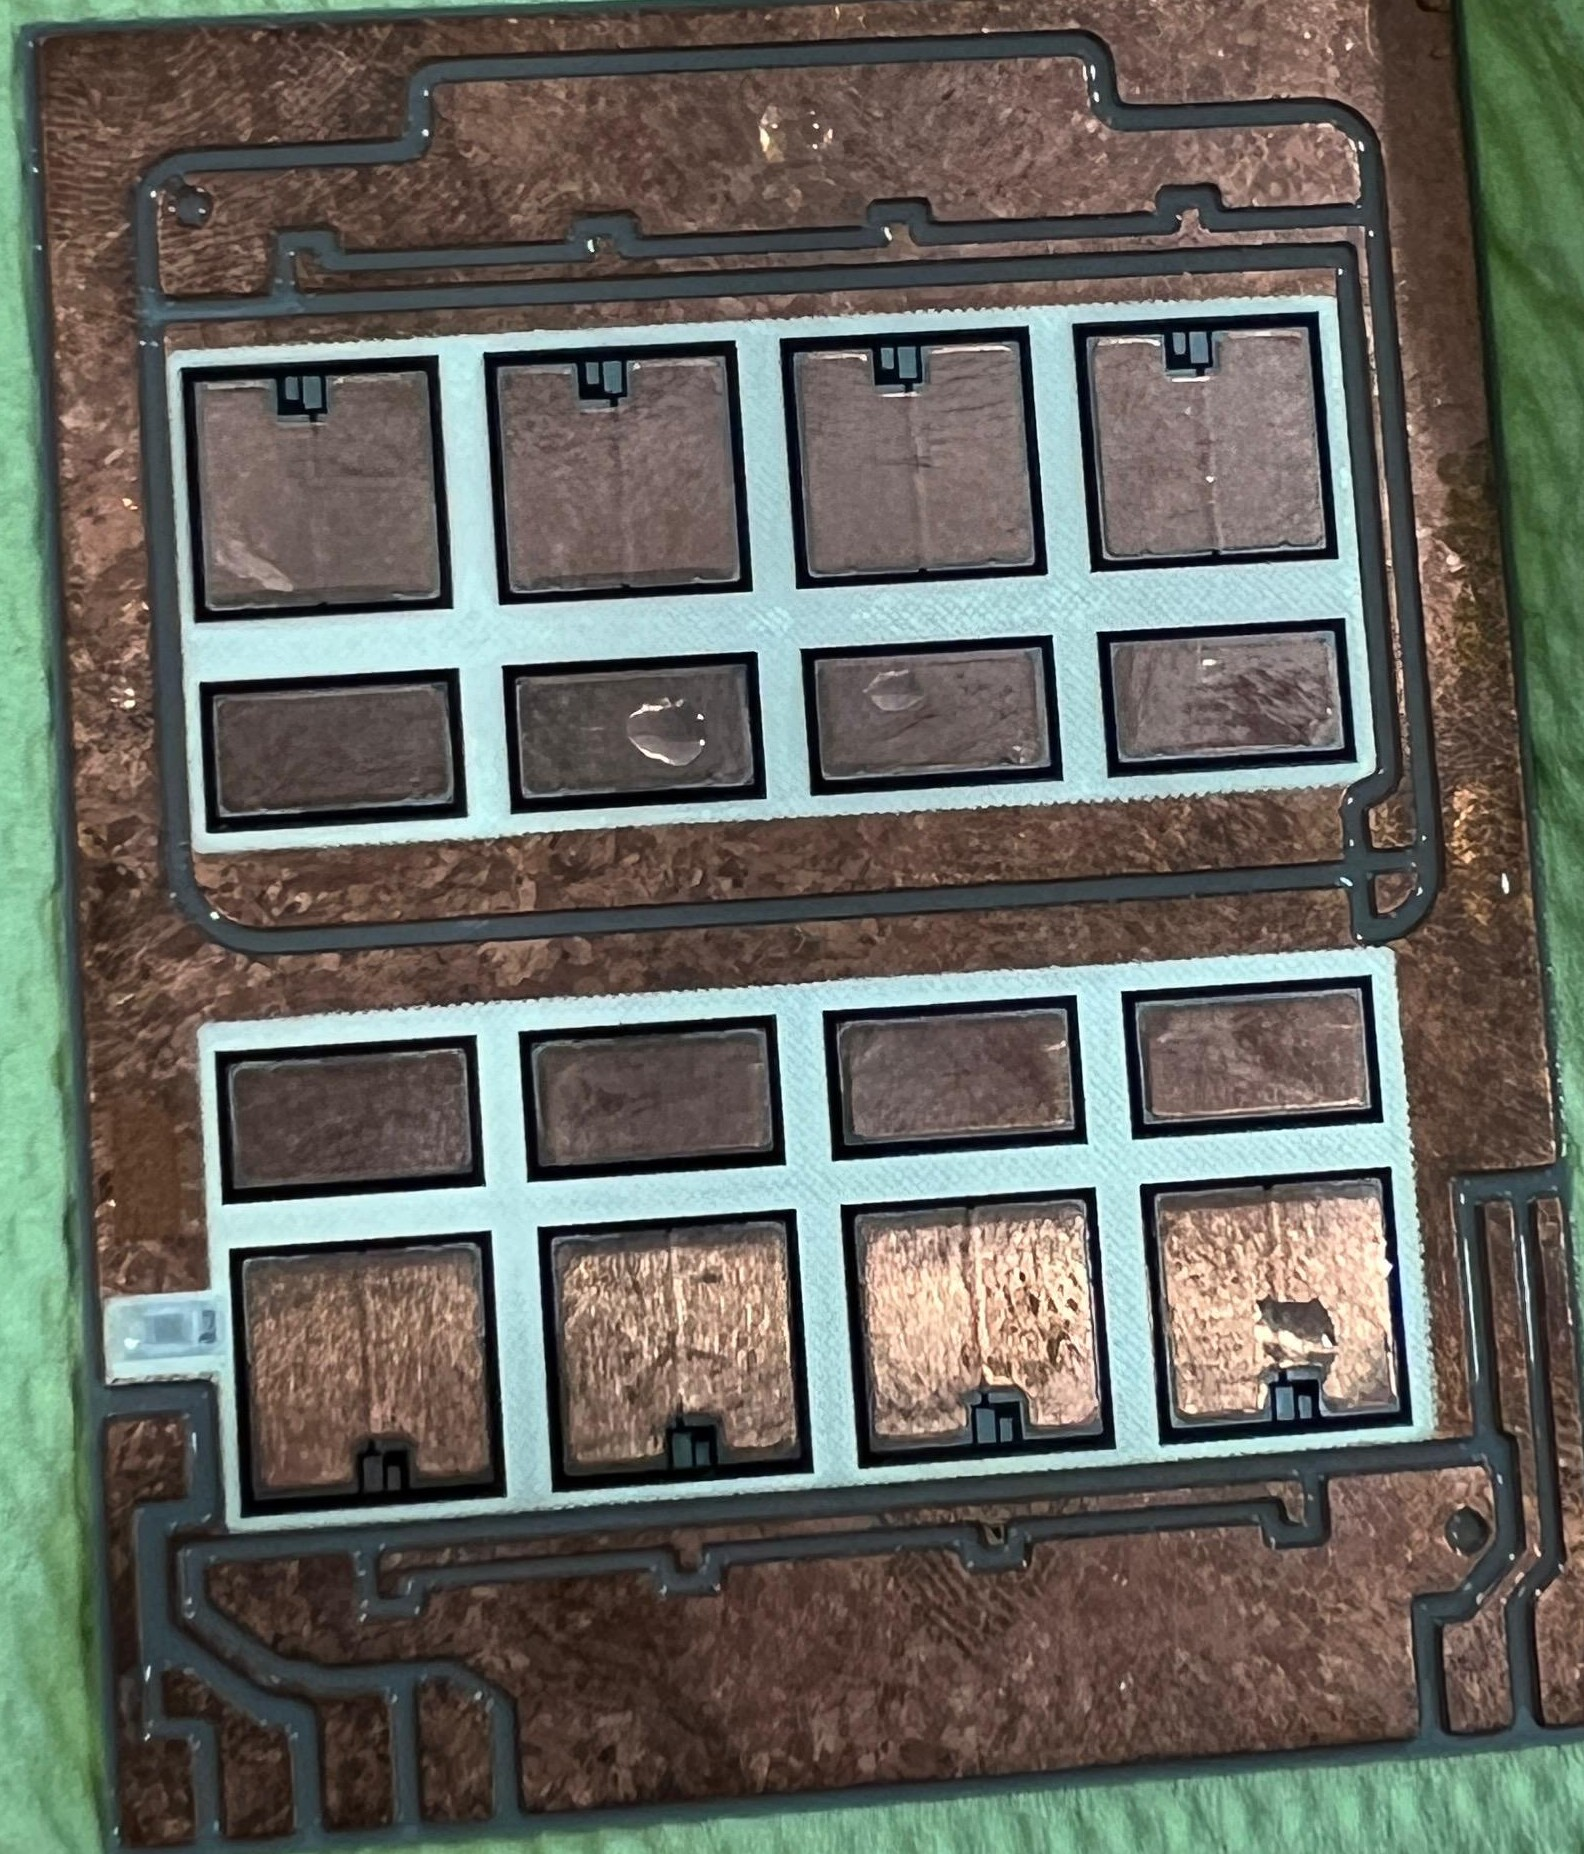
\includegraphics[scale=0.12]{Bilder/probe1}
    \caption{DCB-Leiterplatte mit gesinterten Halbleitern und teilweiser Kontaktierung durch Bonddrähte. Die Probe dient zur Einarbeitung in die Bedienung des akustischen Mikroskops sowie zur Analyse von Materialübergängen.}
    
    \vspace{0.2cm}
    \label{Abb.3: DCB-Leiterplatte mit gesinterten Halbleitern und teilweiser Kontaktierung durch Bonddrähte. Die Probe dient zur Einarbeitung in die Bedienung des akustischen Mikroskops sowie zur Analyse von Materialübergängen. }
\end{figure} 
\vspace{0.2cm}
\begin{figure}[htbp]
    \centering
    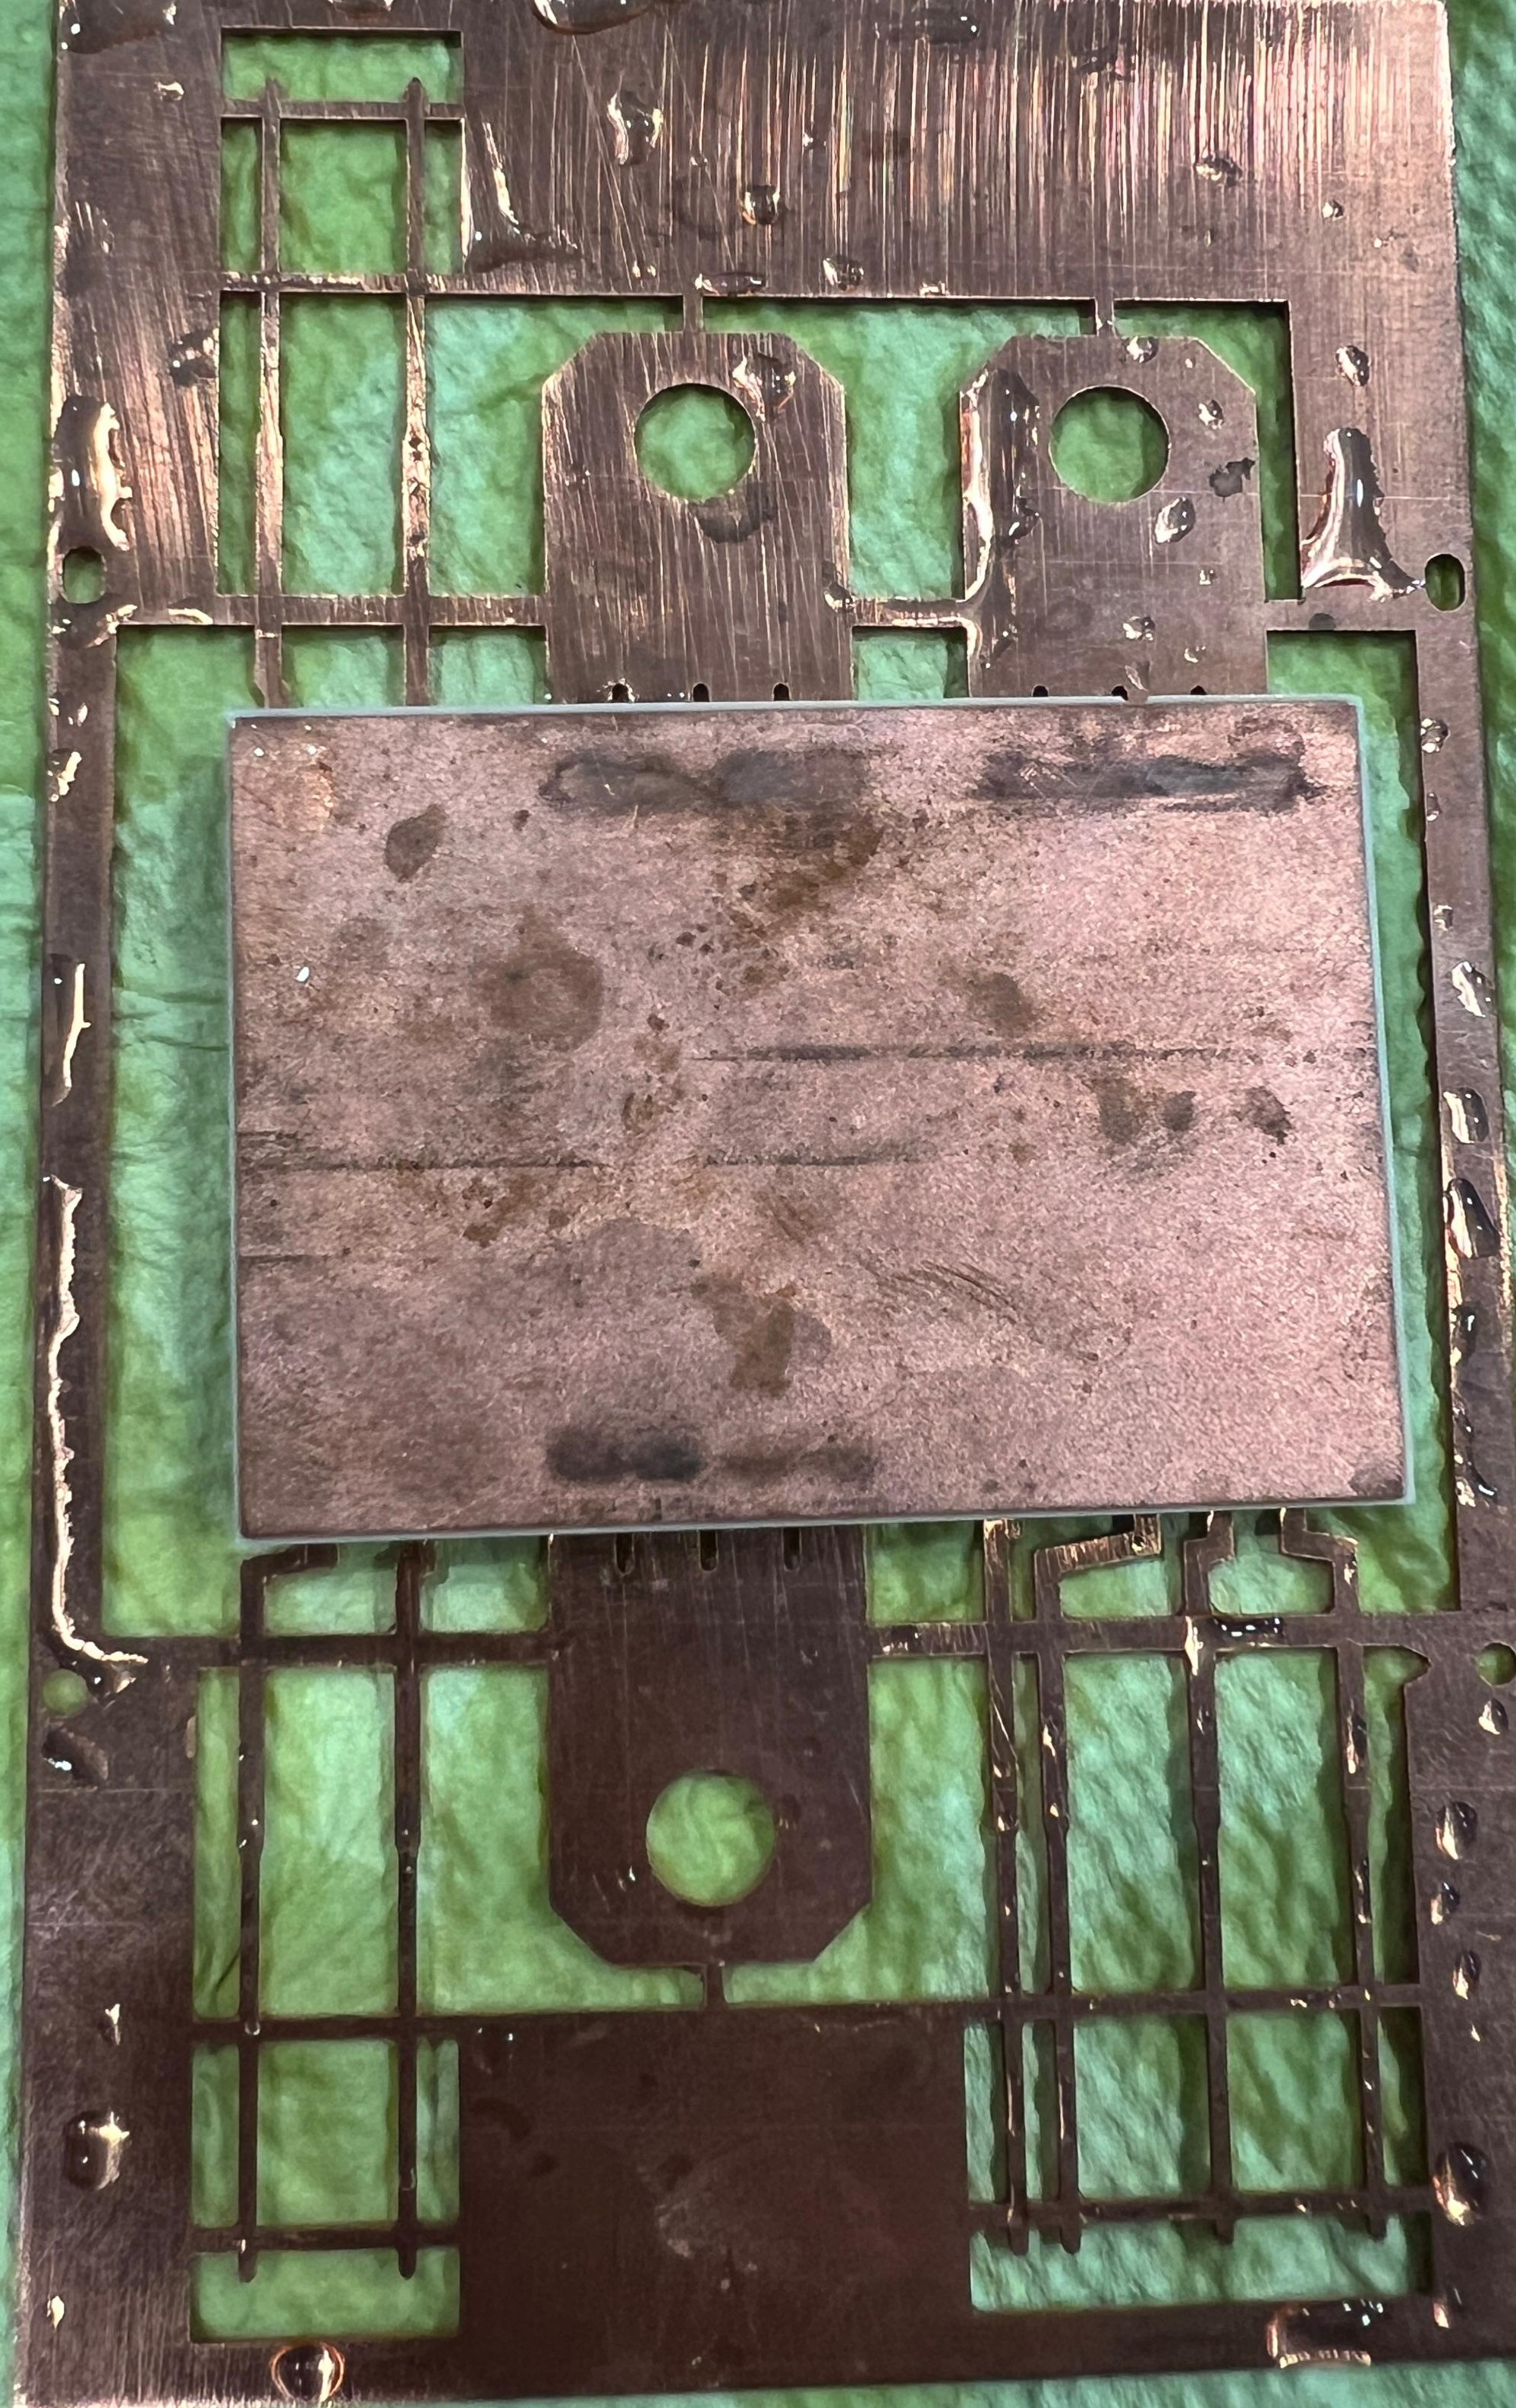
\includegraphics[scale=0.12]{Bilder/probe 2}
    \caption{Keramisches Substrat mit angeschweißtem Kupfer-Leadframe. Die Untersuchung konzentriert sich auf die Qualität der Schweißverbindungen und das Auffinden potenzieller Defekte.}
    \vspace{0.2cm}
    \label{Abb.4: Keramisches Substrat mit angeschweißtem Kupfer-Leadframe. Die Untersuchung konzentriert sich auf die Qualität der Schweißverbindungen und das Auffinden potenzieller Defekte. }
\end{figure} 
\vspace{0.2cm}
\begin{figure}[htbp]
    \centering
    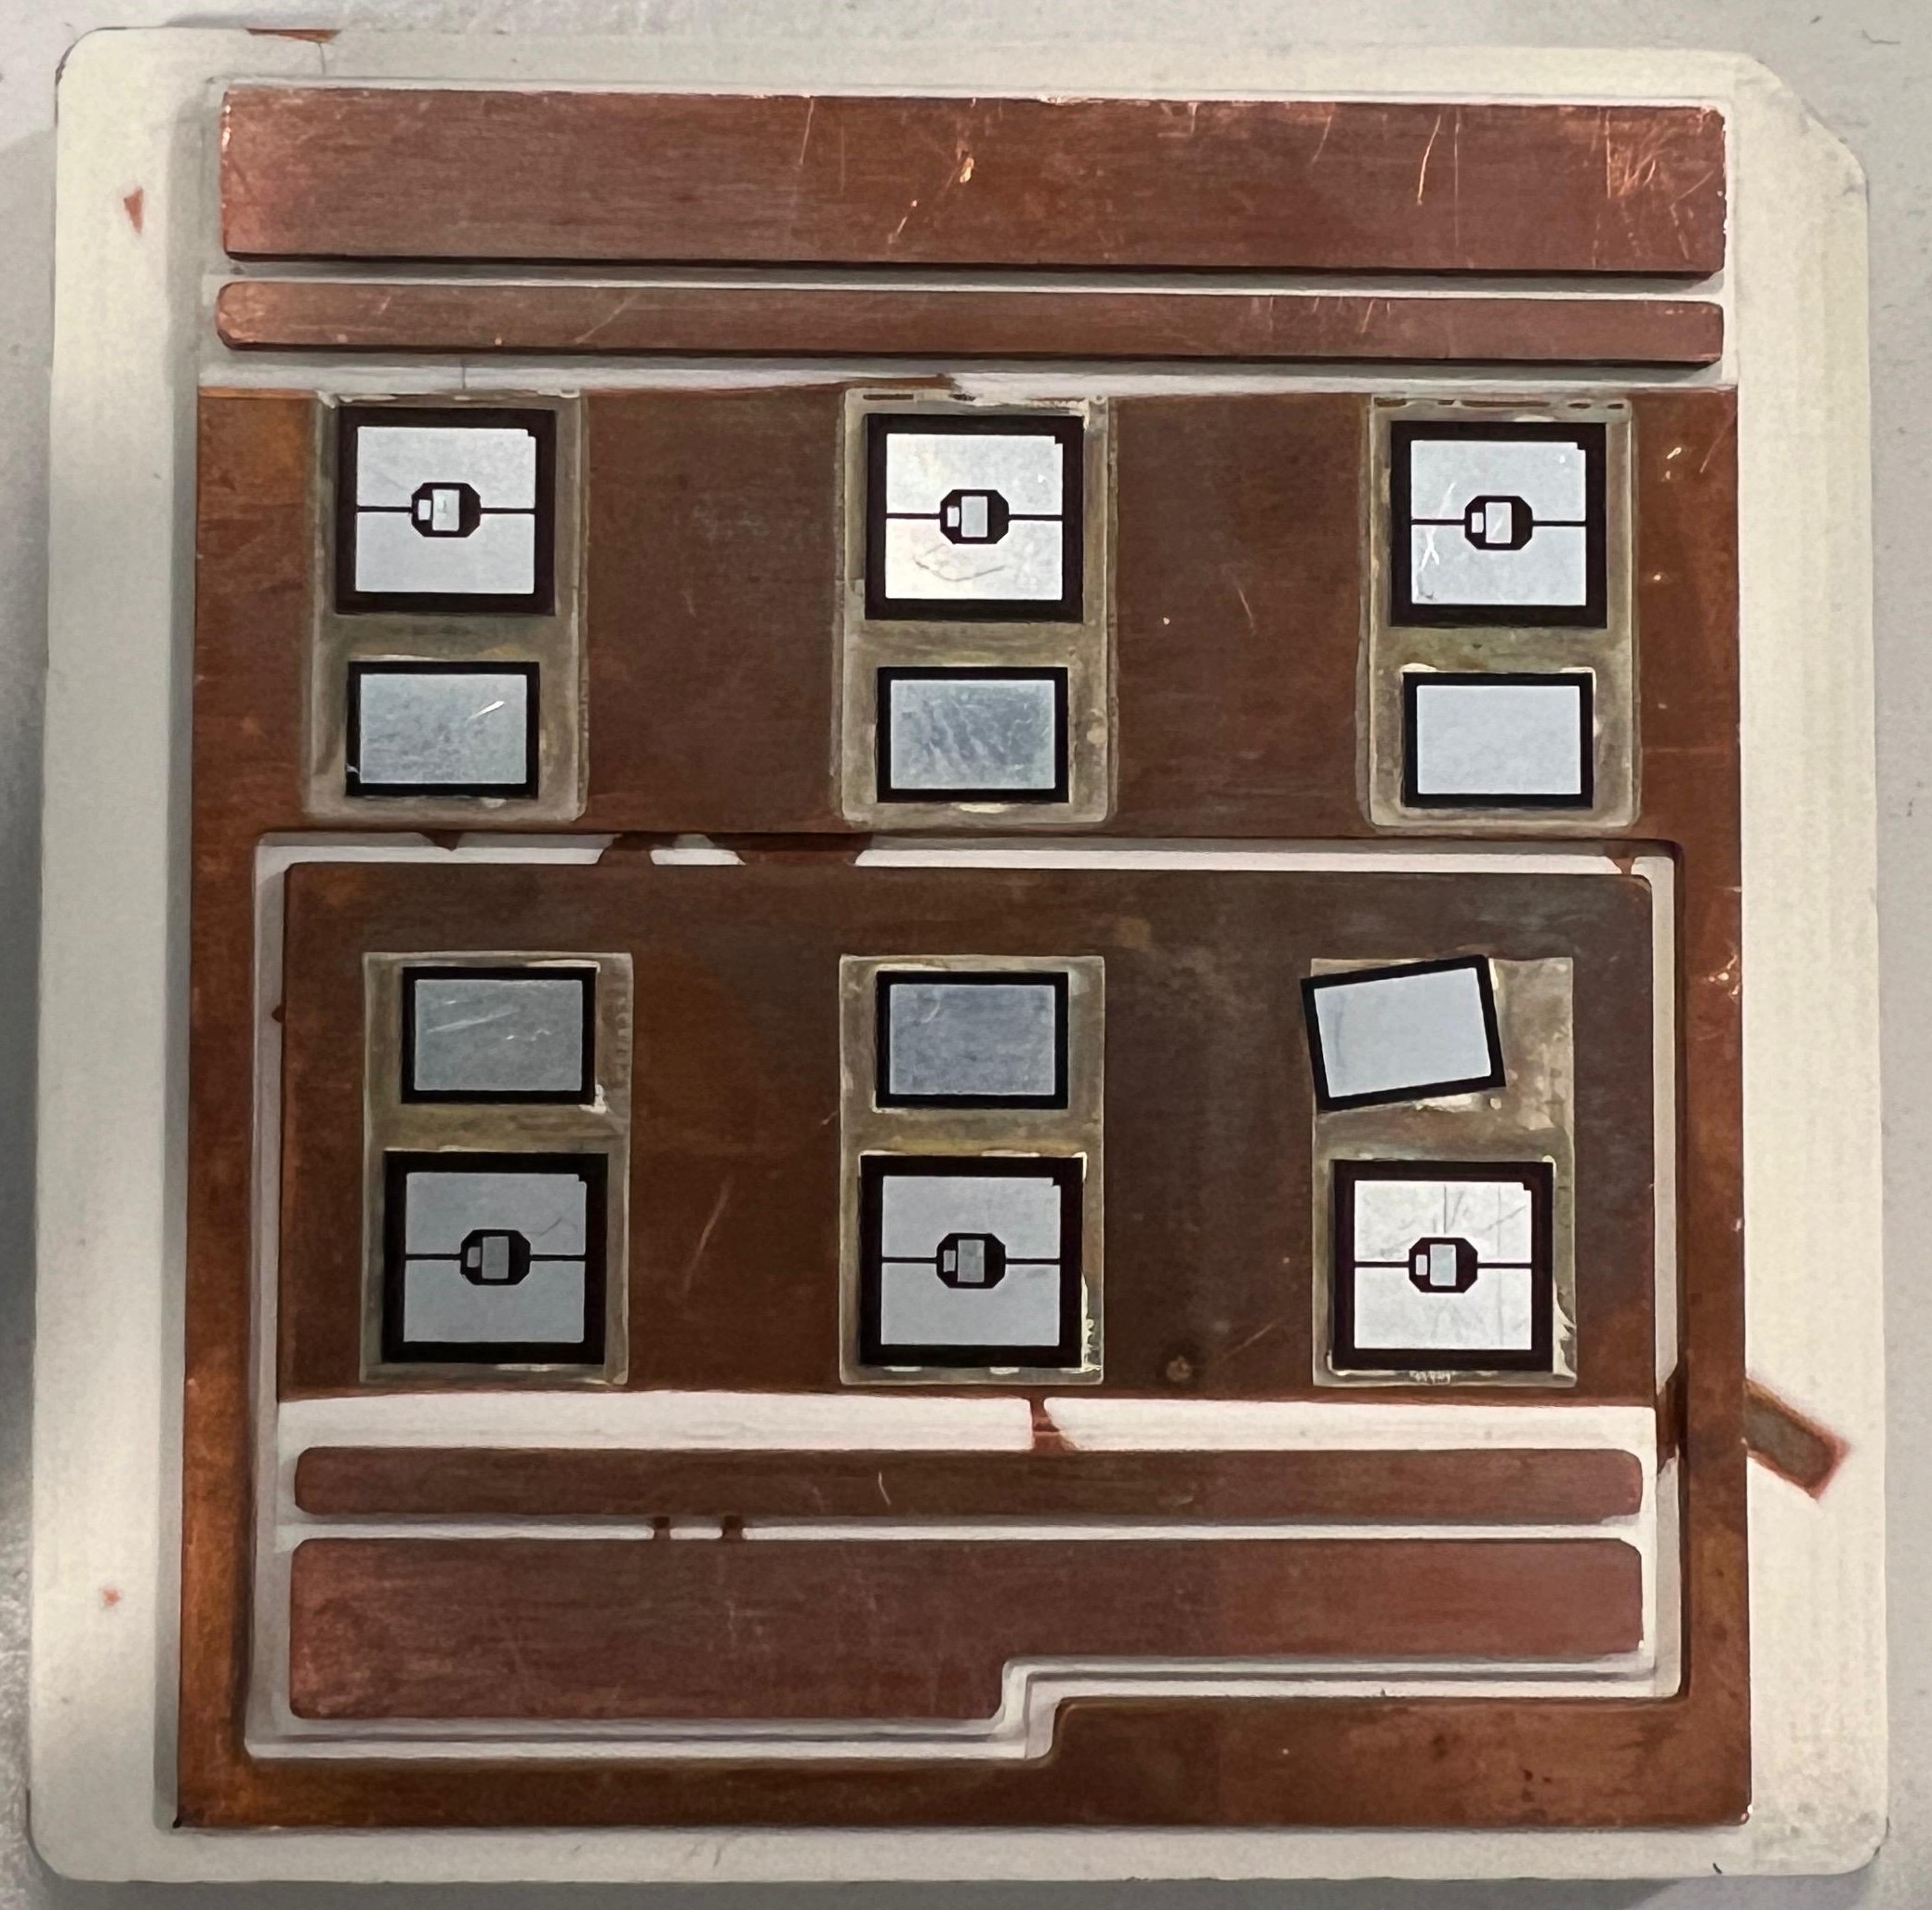
\includegraphics[scale=0.13]{Bilder/probe3}
    \caption{DoL-Leistungselektronikmodul ohne Bonddrähte. Statt keramischer Isolation kommt eine organische Trägerfolie zum Einsatz. Ziel ist die eigenständige Auswahl und Bewertung geeigneter Fokusebenen.}
    \vspace{0.2cm}
    \label{Abb.5: DoL-Leistungselektronikmodul ohne Bonddrähte. Statt keramischer Isolation kommt eine organische Trägerfolie zum Einsatz. Ziel ist die eigenständige Auswahl und Bewertung geeigneter Fokusebenen. }
\end{figure} 
\vspace{0.2cm}

%------------------------------------------------------
%######################################################
%------------------------------------------------------
\clearpage
\section{Durchführung}
\input{Sections/05-Durchführung}


%------------------------------------------------------
%######################################################
%------------------------------------------------------

\section{Ergebnisse}
\subsection{Probe 1}

Die erste Probe zeigt eine gleichmäßige, klar abgegrenzte Struktur mit regelmäßig angeordneten quadratischen Elementen (siehe Abbildung~\ref{Abbildung 6 :probe1}). Die Reflexionssignale erscheinen homogen, ohne sichtbare Unterbrechungen oder Unregelmäßigkeiten innerhalb der Materialübergänge. Auffällig ist die hohe Signalklarheit in den bondfreien Zonen. Es lassen sich weder Risse noch Delaminationen erkennen, was auf eine saubere Verarbeitung und intakte Schichten schließen lässt.
\vspace{0.2cm}
\begin{figure}[htbp]
    \centering
    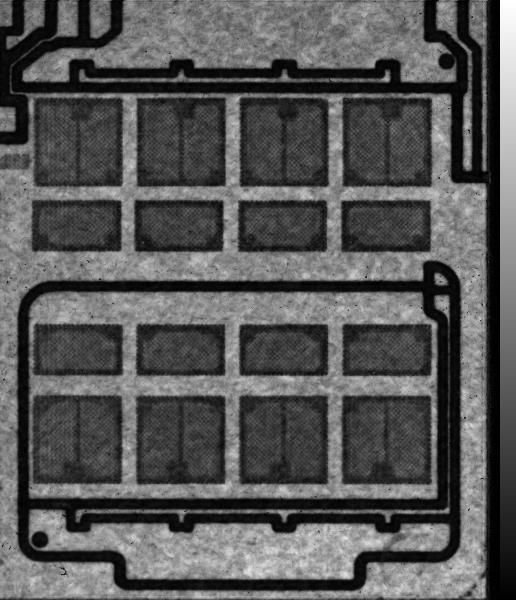
\includegraphics[scale=0.20]{Bilder/Probe11.jpg}
    \caption{C-Scan der Probe 1 mit klar erkennbaren Strukturen und homogener Reflexion.}
    \label{Abbildung 6 :probe1}
\end{figure}
\vspace{0.5cm}
\subsection{Probe 2}
Bei der zweiten Probe wird eine Schicht-für-Schicht-Analyse durchgeführt. In den insgesamt fünf Fokusebenen zeigen sich deutliche Unterschiede in der Signalintensität und den erkennbaren Strukturen. Die obersten Ebenen (Abbildung~\ref{Abbildung 7_1:probe2_1} und \ref{Abbildung 7_2:probe2_2}) erscheinen relativ glatt, wobei eine kreisförmige Auffälligkeit in Form eines dunklen Punktes sichtbar ist. Dies könnte auf eine Lufteinschluss oder lokale Delamination hindeuten.

Mit zunehmender Tiefenlage (Abbildung~\ref{Abbildung 8_1:probe2_3} bis \ref{Abbildung 8_2:probe2_4}) treten vermehrt Leiterstrukturen hervor, die in den oberen Schichten nicht sichtbar waren. Zudem zeigen sich in tieferen Ebenen leichte Schattenbildungen und Signalbrüche entlang einzelner Linien, was auf potenzielle Trennungen oder Materialunregelmäßigkeiten in unteren Bondschichten hinweist.
\vspace{0.2cm}
\begin{figure}[htbp]
    \centering
    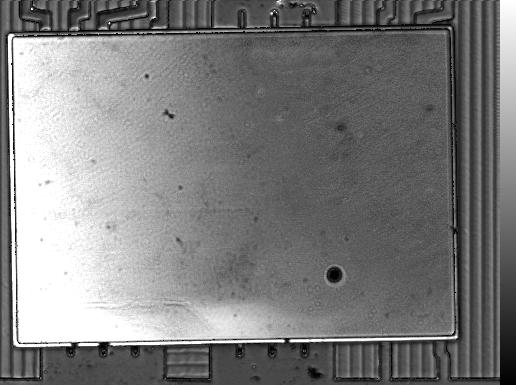
\includegraphics[scale=0.30]{Bilder/Probe2_i794_x001.jpg}
    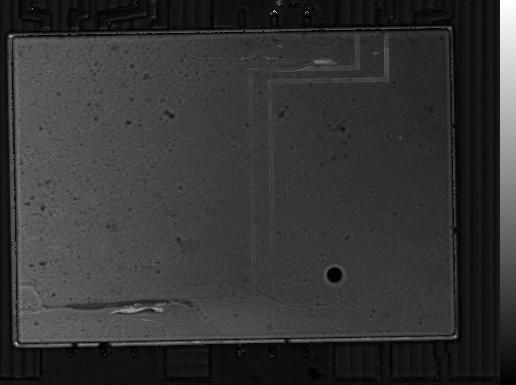
\includegraphics[scale=0.30]{Bilder/Probe2_i794_x002.jpg}
    \caption{Obere Fokusebenen der Probe 2. Die rechte Abbildung zeigt eine auffällige Reflexionsunterbrechung.}
    \label{Abbildung 7_1:probe2_1}
    \label{Abbildung 7_2:probe2_2}
\end{figure}

\begin{figure}[htbp]
    \centering
    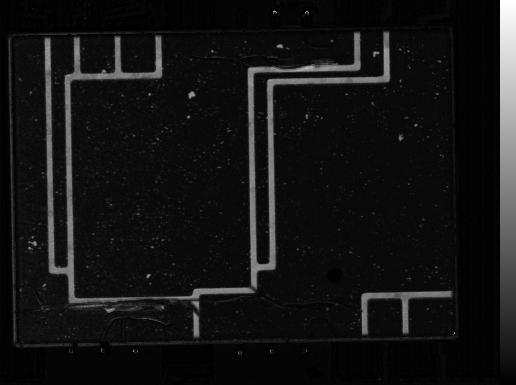
\includegraphics[scale=0.30]{Bilder/Probe2_i794_x003.jpg}
    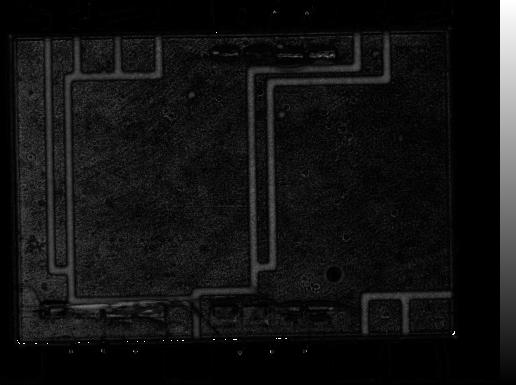
\includegraphics[scale=0.30]{Bilder/Probe2_i794_x004.jpg}
    \caption{Mittlere Fokusebenen der Probe 2 mit zunehmender Sichtbarkeit der Leiterstrukturen.}
    \label{Abbildung 8_1:probe2_3}
    \label{Abbildung 8_2:probe2_4}
\end{figure}
\clearpage
\begin{figure}[htbp]
    \centering
    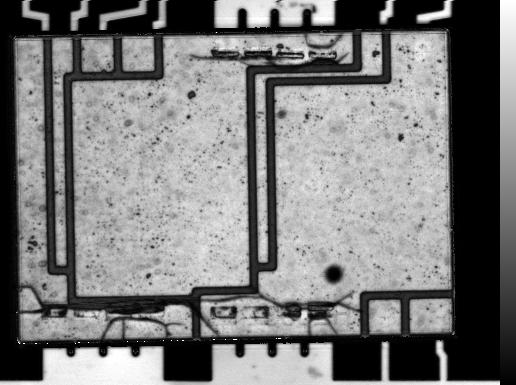
\includegraphics[scale=0.30]{Bilder/Probe2_i794_x005.jpg}
    \caption{Tiefste gescannte Ebene der Probe 2. Sichtbare Leiterbahnen mit lokalen Unregelmäßigkeiten im unteren Bereich.}
    \label{Abbildung 9:probe2_5}
\end{figure}


\subsection{Probe 3}

In der letzten Probe, einem DoL-Modul, fällt sofort die großflächige, glatte Reflexionsfläche auf (siehe Abbildung~\ref{Abbildung 10:probe3}). Die Struktur wirkt weitgehend homogen. Es sind keine offensichtlichen Risse oder Hohlräume erkennbar. Bemerkenswert ist jedoch die gute Lesbarkeit des Schriftzugs \enquote{FH-KIEL} in der Bildmitte. Dies deutet auf eine hohe Oberflächengüte und gleichmäßige Signalreflexion hin.
\vspace{0.2cm}
\begin{figure}[htbp]
    \centering
    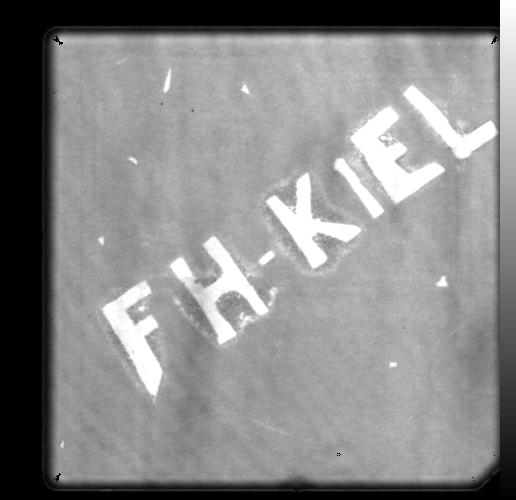
\includegraphics[scale=0.30]{Bilder/Probe3_i795_c.jpg}
    \caption{C-Scan der Probe 3 (DoL-Modul) mit gleichmäßiger Reflexionsfläche und klar erkennbarer Gravurstruktur.}
    \label{Abbildung 10:probe3}
\end{figure}



%------------------------------------------------------
%######################################################
%------------------------------------------------------
\clearpage
\section{Zusammenfassung}

Im Rahmen des Versuchs zur akustischen Mikroskopie wurden drei unterschiedliche Proben untersucht: ein DCB-Modul mit gesinterten Halbleitern, ein geschweißter Kupfer-Leadframe auf Keramik sowie ein DoL-Leistungselektronikmodul mit organischer Trägerfolie. Ziel ist es, mithilfe des C-Scan-Modus im Reflexionsverfahren die inneren Materialschichten und Grenzflächen zerstörungsfrei zu analysieren und visuell darzustellen.

Die Untersuchungen erfolgten in mehreren Fokusebenen, insbesondere bei der zweiten Probe, um strukturbedingte Unterschiede sichtbar zu machen. Das verwendete KSI V8 SAM ermöglichte dabei hochauflösende Aufnahmen, aus denen potenzielle Defekte, Delaminationen und Unregelmäßigkeiten abgeleitet werden konnten.\\
Die Ergebnisse zeigen, dass das DoL-Modul (Probe 3) weitgehend homogen aufgebaut ist und keine auffälligen strukturellen Defekte aufweist. Lediglich einige mögliche Oberflächenverunreinigungen oder Lufteinschlüsse sind erkennbar. Auffällig ist die klar lesbare Gravur „FH-KIEL“, was auf eine gute Oberflächenreflexion und geringe Dämpfung hindeutet.

Bei der ersten Probe (DCB-Modul) konnten keine Risse oder Delaminationen festgestellt werden. Die Draht-Bonds erscheinen vollständig intakt, und die Kontaktierungen zwischen den Kupferflächen sind klar sichtbar. Die zweite Probe (Leadframe auf Keramik) offenbarte bei der schichtweisen Untersuchung einzelne Unregelmäßigkeiten in tieferen Ebenen. Diese deuten auf Schwachstellen in der Materialanbindung hin, insbesondere entlang der unteren Bondschicht.

%------------------------------------------------------
%######################################################
%------------------------------------------------------

\section{Fazit}

Der Versuch verlief reibungslos und zeigte, dass die akustische Mikroskopie mit dem KSI V8 SAM eine effektive und zuverlässige Methode zur zerstörungsfreien Prüfung innerer Strukturen darstellt. Die gewonnenen Erkenntnisse bilden eine fundierte Basis für die Beurteilung der Materialqualität und können zur Optimierung von Fertigungsprozessen in der Leistungselektronik beitragen.


%------------------------------------------------------
%######################################################
%------------------------------------------------------

%\section{Formelzeichen}
%\input{Sections-ending/09-Formelzeichen}

%------------------------------------------------------
%######################################################
%------------------------------------------------------



%------------------------------------------------------
%######################################################
%------------------------------------------------------
\newpage

\listoffigures

%------------------------------------------------------
%######################################################
%------------------------------------------------------



%------------------------------------------------------
%######################################################
%------------------------------------------------------

\section{Literaturverzeichnis}
\printbibliography[]

%------------------------------------------------------
%######################################################
%------------------------------------------------------

%------------------------------------------------------
%######################################################
%------------------------------------------------------


%------------------------------------------------------
%--------------------Vorlage-Testing-------------------
%------------------------------------------------------

%\section{Vorlage-Testing}
%\input{Vorlage/Figuren-Struktur}
%\input{Vorlage/Tabellen-Struktur}


\newpage

\end{document}